\newpage
\section{Постановка задачи}

\begin{flushleft}
	Исследование из области солнечной энергетики. На Рис.1 показана схема установки для исследования фотоэлектрических характеристик.
\end{flushleft}
\begin{figure}[H]
	\center{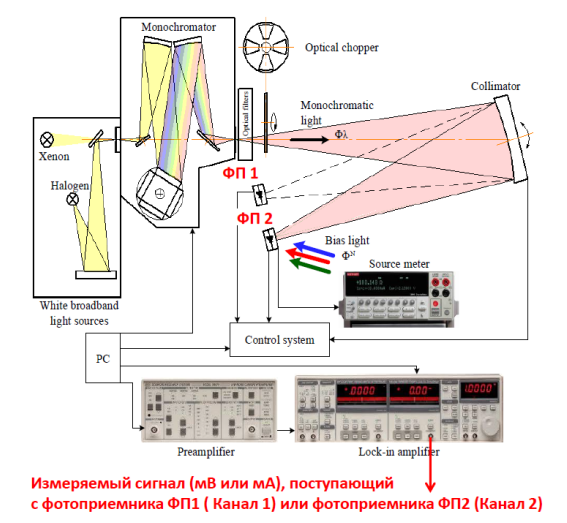
\includegraphics[width=1\linewidth]{images/shcema}}
	\caption{Схема установки}
	\label{fig:shcema}
\end{figure}
\begin{flushleft}
	Калибровка датчика ФП1 производится по эталону ФП2. Зависимость между квантовыми эффективностями датчиков предполагается постоянной для каждой пары наборов измерений
	\begin{equation}
		QE_{ФП2}\,=\,\frac{I_{ФП2}}{I_{ФП1}}*QE_{ФП1}.
		\label{1}
	\end{equation}
	$QE_{ФП1,2}\,-$ квантовые эффективности эталонного и исследуемого датчиков, $I_{ФП1,2}\,-$ измеренные токи.\\
	\textbf{Исходные данные:} Имеется 2 выборки данных с интервальной неопределенностью. Одна из них относится к эталонному датчику ФП2. Другая выборка соответствует исследуемому датчику ФП2. Данные представлены в виде двух csv файлов с числом отсчетов 200.\\
	\vspace{0.5em}
	\textbf{Требуется определить:} коэффициент калибровки
	\begin{equation}
		R_{21}\,=\,\frac{I_{2}}{I_{1}}.
		\label{2}
	\end{equation}
	при помощи линейной регрессии на множестве интервальных данных и коэффициента Жаккара.
\end{flushleft}